\documentclass{article}
\usepackage[utf8]{inputenc}

\title{}


\title{%
  Text Mining for Information Retrieval on WikIR \\
  \large Project for Machine Learning course}
\author{Jakub Bartczuk}
\date{Winter 2020}

\usepackage{natbib}
\usepackage{graphicx}
\usepackage{url}
\usepackage{hyperref}

\begin{document}

\maketitle

\section{Motivation}
One of the first things that data scientists do when facing a new problem is searching for related problems and software on GitHub. GitHub's search capabilities are very limited (at the time of writing this report) - there are several features like project descriptions, tags and readmes that could be helpful, but its search engine doesn't allow for searching them simultaneously. The effect is that sometimes reformulating query might result in drastically different search results. This project aims at evaluating in a controlled experiment several simple text mining methods that can be useful for expanding traditional bag-of-words retrieval model.

\section{Abstract}

WikIR \citep{frej2019wikir} is a recently proposed dataset for evaluating Information Retrieval. So far it was used only to benchmark standard Information Retrieval method (BM25)\citep{manning2008introduction} versus deep learning-based text matching. In this project several machine learning methods for text, using classification, word embeddings and matrix decomposition were used to improve searching results.

\section{Dataset}
The dataset consists of approx. 100k documents and queries split into training, validation and test sets (with 1k, 100 and 100 examples respectively). It is created from wikipedia articles and their titles: queries are the titles, whereas rest of article (with first paragraph removed) gets split into 'documents' to be retrieved. Document is deemed relevant for query if either the query is the title of document's article (relevance score 2) or its article is linked in retrieved document's article. Below query lengths are reported. Document lengths are less interesting, since author's method splits articles into documents of approx. 200 words.

\begin{figure}[h!]
\centering
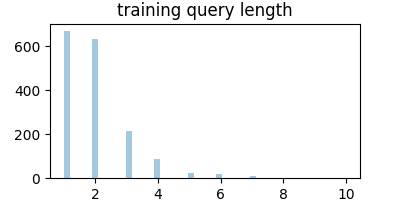
\includegraphics[scale=1.1]{images/training_query_length.png}
\label{fig:universe}
\end{figure}

\begin{figure}[h!]
\centering
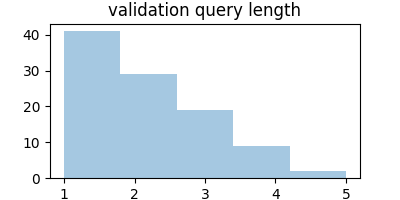
\includegraphics[scale=1.1]{images/validation_query_length.png}
\label{fig:universe}
\end{figure}

\begin{figure}[h!]
\centering
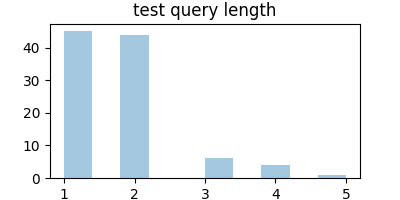
\includegraphics[scale=1.1]{images/test_query_length.png}
\label{fig:universe}
\end{figure}

\section{Evaluation}

All methods apart from query expansion-based retriever first retrieve 100 records using BM25 relevance model and then perform reranking.

Results are evaluated using standard Information Retrieval metrics: Precision at $k$, nDCG at $k$ and Mean Average Precision.

\section{Data preparation} 
For our models we preprocess data according to original paper: english stop words are removed and the words are stemmed using Porter stemmer. These steps are performed using NLTK \citep{Loper02nltk:the}.

Models were tested with both stemmed and unstemmed texts. Also, keyword extraction was used as a step for some word embedding models (to alleviate problem of averaging larege documents). Keyword extraction was performed using gensim's \citep{rehurek_lrec} textrank model.

\section{Models}
 
\begin{enumerate}
  \item Classification on BM25 features and tf-idf features \citep{DBLP:journals/corr/abs-1904-08861}
  \item Classification on using GloVe \citep{Pennington14glove:global} and FastText \citep{bojanowski2016enriching}  word embeddings 
  \item Scoring using similarity based on unsupervised representation (using Nonnegative Matrix Factorization)
  \item Query expansion using nearest words using word embeddings.
  
Models 1-3 work by combining their score with relevance score. BM25 model is first used to retrieve 100 top documents. Model score results from running classification: top $k$ are defined as positive and bottom $k$ documents are defined as negative.
  
\end{enumerate}

\section{Results}

\section{Deliverables}

Project's code can be found on its GitHub page\footnote{\href{https://github.com/lambdaofgod/wikir_text_mining}{https://github.com/lambdaofgod/wikir_text_mining}}.

\section{Conclusion}
BM25 already provides strong baseline for search results ranking. The difference noted in Lin's paper (metod beating BM25 by 2\% MAP) doesn't happen for WikIR, most likely because of the fact that WikIR queries are very short so retrieval is almost 'all or nothing'. It remains an open question whether the results can be improved by using simple machine learning models on top of features extracted using pretrained language models.

\section{Further steps}
\begin{itemize}
    \item use word embedding features for global search - there are methods for building large scale approximate kNNs. These might alleviate query vocabulary mismatch problem.
    \item use language-model based features
    \item use Learning to Rank approach
    \item use dataset construction method on another source
\end{itemize}

\bibliographystyle{plain}
\bibliography{references}
\end{document}